% =====================================================================
% R4 supplementary material - Cyber Security and Applications
% Every paragraph sits on one line. Tables in tables/ are generated by
% make_tables.py from the raw CSV files; do not edit them by hand.
% Build:  python3 make_tables.py && latexmk -pdf supplementary.tex
% =====================================================================
\documentclass[10pt]{article}
\usepackage[letterpaper,margin=1in]{geometry}
\usepackage{amsmath,amssymb}
\usepackage{booktabs,array,longtable}
\usepackage{graphicx}
\usepackage{xcolor}
\usepackage{caption}
\usepackage{float}
\usepackage[hidelinks]{hyperref}
\usepackage{url}
\captionsetup{font=small,labelfont=bf}
\renewcommand{\thetable}{S\arabic{table}}
\renewcommand{\thefigure}{S\arabic{figure}}
\renewcommand{\thesection}{S\arabic{section}}
\renewcommand{\thesubsection}{S\arabic{section}.\arabic{subsection}}
\setlength{\parskip}{3pt}
\setlength{\emergencystretch}{3em}
% Fill these two once the repository is public and archived.
\newcommand{\repourl}{\textcolor{red}{[GitHub URL]}}
\newcommand{\zenodo}{\textcolor{red}{[Zenodo DOI]}}

\title{Supplementary material for\\[2pt] \large Full-Mode Implementation of the 3GPP 256-NCA4, 256-NCA5 and 256-NCA6 Algorithms for 6G: Packet-Size, Energy and Constant-Time Evaluation on Microcontroller, ARM, x86 and FPGA}
\author{Sohel Rana and Md. Rubaiyat Hossain Mondal\\[2pt]\small Institute of Information and Communication Technology (IICT)\\\small Bangladesh University of Engineering and Technology (BUET), Dhaka, Bangladesh}
\date{}

\begin{document}
\maketitle

\section{About this supplement}
\label{sec:s-about}

This supplement extends the main paper. It gives the method details, results, tables and figures that do not fit in the page limit of the paper. Section~\ref{sec:s-method} adds method details. Section~\ref{sec:s-results} gives the full results of every tier, with all three modes, all levels and all packet sizes. Section~\ref{sec:s-env} lists the software and hardware environment. Section~\ref{sec:s-artifact} describes the public code and data package and shows which script produces each figure and table.

Every number in this supplement comes from a raw CSV file of the measurement campaign. The script \texttt{paper/supplementary/make\_tables.py} builds all tables of Section~\ref{sec:s-results} from these files, so no table cell is typed by hand. Each caption names its source file. The package is available at \repourl{} and archived at \zenodo{}.

\section{Extended method}
\label{sec:s-method}

\subsection{The 256-AEAD1 interface in our code}

All implementations share one interface with three operations, as in the specification. The first operation, \texttt{init}, loads the 256-bit key and the 128-bit IV and runs the initialization of the core. The second, \texttt{genHQP}, produces the three 128-bit MAC keys $H$, $Q$ and $P$. The third, \texttt{genKS}, produces keystream in 16-byte blocks. The IV comes from Make\_5GIV. It packs the 32-bit COUNT, the 5-bit bearer, the direction bit, six bytes reserved for future entropy, the tag length and two flags. One flag separates 256-NCA from 256-NEA and 256-NIA. The other separates the generation of $H$, $Q$ and $P$ from the keystream. A 256-NCA call therefore runs one initialization, one \texttt{genHQP} and the keystream for the message. A 256-NEA call plus a separate 256-NIA call runs two initializations, because each uses its own IV. This is the reason why the combined mode saves work for short packets (main paper, Section~7).

\subsection{Implementation details}

At L2 and L3, we produce the keystream in chunks of 512 bytes. We compute the MAC over each chunk of ciphertext while it is still in the first-level cache. The POLYVAL part absorbs eight blocks per reduction at L2, with the powers $H$ to $H^8$ computed once per packet. At L3 it absorbs sixteen blocks per reduction with 512-bit carry-less multiplication. Below 512 bytes, the L3 code calls the L2 code. We set this threshold from the Zen~4 data, where the 512-bit setup cost more than it saved for short packets.

For Snow~5G at L2, each 16-cell shift register sits in two 128-bit vector registers. One clock then updates eight cells at once, and the two AES rounds of the state machine use the AES instruction. On the Pi~5, unrolling the Snow~5G loop by four clocks lowers its keystream cost by 10\%. For AES-256 on the Pi~5, our first version expanded the key with the table look-ups of L1 and needed 1641 cycles for an empty 256-NCA5 packet. We now expand the key with the AES instruction, which cuts this cost to 721 cycles, a factor of 2.3. For ZUC-256, we keep the 16-cell register as a ring inside a 16-step unrolled loop, so no cell moves in memory.

The constant-time ZUC-256 (levels L2ct and L3ct) replaces only the S-box layer. The layer computes $S_0[x_{31..24}] \| S_1[x_{23..16}] \| S_0[x_{15..8}] \| S_1[x_{7..0}]$. The table code reads $S_0$ and $S_1$ from memory at addresses that depend on the key, and this leaks (main paper, Section~5.8). The new code keeps both 256-byte tables in vector registers. On Zen~4, one \texttt{VPERMI2B} selects bytes from 128 table entries. Two of them cover 256 entries, and bit~7 of each index chooses the half. On the Pi~5, one \texttt{TBL} selects bytes from 64 entries and returns zero outside them. Four of them cover 256 entries, with the index lowered by 64 each time, and the four results are ORed. The code looks up both $S_0$ and $S_1$ for all four bytes, and a constant byte mask keeps $S_0$ in bytes 3 and 1 and $S_1$ in bytes 2 and 0. Neither the instruction stream nor any memory address then depends on the key. The constant-time code needs AVX-512 VBMI on x86.

\subsection{Measurement protocol details}

For each point, the harness first times three trial batches and takes the fastest. It then sets the batch size so that one batch lasts at least 2~ms. Five warm-up batches and 31 timed batches follow. Each batch calls the same function on the same buffers, with the packet counter COUNT increased for every call, so every call runs a full initialization. The input buffer starts on a page boundary, and the output buffer starts 2048 bytes into a page. The CSV header records this layout (\texttt{in\_mod4096=0}, \texttt{out\_mod4096=2048}). Section~\ref{sec:s-layout} shows the effect of other layouts.

On Zen~4 and the Pi~5, the harness reads core cycles with the Linux \texttt{perf\_event} interface and wall-clock time with \texttt{CLOCK\_MONOTONIC\_RAW}. On Zen~4, it also reads the time-stamp counter. The scripts \texttt{clock\_lock.sh} and \texttt{clock\_restore.sh} set the performance governor, fix the minimum and maximum clock, turn off boost and allow user access to the cycle counter. On the ESP32, the harness reads the CCOUNT register and the 1~$\mu$s timer of ESP-IDF. It runs as the only task on core~1, with the radios never started. All measured code sits in internal RAM through a linker fragment, and the tables sit in internal data RAM.

\subsection{Multi-core runs}

The script \texttt{run\_mc.sh} reads the CPU topology from \texttt{sysfs}. It lists one logical CPU per physical core, ordered by core number, with core~0 last, because core~0 takes most interrupts. It then runs 1, 2, 4 and 8 threads on separate physical cores, and on Zen~4 a final run with all 16 logical CPUs. Each thread has its own key context, buffers and packet counter. Before timing, every thread computes the tag of one reference packet, and a checker compares the tags of all threads. For the OpenSSL test with a fetched cipher object, each thread calls \texttt{EVP\_CIPHER\_fetch} once and then \texttt{EVP\_EncryptInit\_ex2} with the fetched object for every packet. The key is thus still set up for every packet, as in the single-core runs.

\subsection{Energy on the Pi~5}

The script \texttt{energy\_pi.py} reads all rails of the power-management chip with \texttt{vcgencmd pmic\_read\_adc}, about 40 times per second, from core~0. The benchmark runs on core~3. For each case, it records a 10-second idle window and then a 10-second window in which \texttt{bench --run-seconds} runs one algorithm and size without pause. The energy per byte is the rise in power over idle times the run time, divided by the number of payload bytes. Each case runs three times, with idle and active windows alternating.

\subsection{Timing-leakage harness}

The program \texttt{ct} follows the dudect method. For every measurement, it draws one of two classes at random and times one 256-NCA call with serializing reads of the counter. It keeps all measurements and applies Welch's $t$-test to all of them and to 100 subsets cropped at increasing percentiles of the timing distribution. It reports the largest $|t|$. The two control implementations compare a 32-byte key with a fixed pattern. The leaky one stops at the first zero byte. The branch-free one always reads all 32 bytes.

\subsection{FPGA test wrapper}

The board test wraps each engine with a UART at 1~Mbaud, block-RAM buffers for input and output, and a cycle counter. The PC script \texttt{hwtest.py} sends one packet with its key, IV fields, mode and lengths. The engine processes the packet from RAM to RAM at full clock speed. The board then returns the output, the tag and the number of cycles between start and done. The 120 functional packets come from the verified L1 code, written to files by \texttt{gen\_vectors}. They cover all three modes, decryption, associated data, every tag length and lengths in bits. Seven timing packets of 0, 40, 576, 1500 and 16384 bytes follow for 256-NCA, plus 16384 bytes for 256-NEA and 1500 bytes for 256-NIA.

\section{Extended results}
\label{sec:s-results}

\subsection{All modes and levels on each processor}

Tables~\ref{tab:s-zen4}, \ref{tab:s-pi5} and~\ref{tab:s-esp32} list the setup, the cost of 40-byte and 1500-byte packets and the long-packet cost of 256-NEA, 256-NIA and 256-NCA for every set and level. Figs.~\ref{fig:s-zen4} to~\ref{fig:s-esp32} show the cost per byte against packet size and the gain of each level. These are the per-tier figures of an earlier version of the paper.

On Zen~4, L3 256-NEA5 is faster than OpenSSL AES-256-CTR at every size we test. The factor is 16.2 for an empty packet and 1.41 for 1~MiB. The cost per byte stays flat from 64~KiB to 1~MiB for every set and level within 1\%, because the 1~MiB buffers still fit in the 32~MiB third-level cache.

On the Pi~5, L2 256-NEA5 is faster than OpenSSL AES-256-CTR up to 9000 bytes, by a factor of 3.1 for an empty packet. From 16 to 64~KiB, AES-256-CTR is 3 to 9\% faster. The 1~MiB point is less stable on this tier. The input and output buffers together take 2~MiB, which exceeds the 512~KiB second-level cache of one core and fills the 2~MiB shared cache. At 1~MiB, the interquartile range rises to 18\% of the median for 256-NEA4 and to 12\% for 256-NCA5, and their medians rise by 12\% and 6\% over the 64~KiB values. The reference schemes ChaCha20-Poly1305 and AEGIS-256 come from a later run. In that run, AES-256-GCM repeats its earlier cost at 64~KiB within 0.1\%, but its fixed cost is 5 to 7\% higher for packets up to 256 bytes.

On the ESP32, HW 256-NEA5 is 1.29 to 2.05 times faster than mbedTLS AES-256-CTR, which uses the same AES engine. The later run with the reference schemes repeats every 3GPP and AES-256-GCM point of the main run within 0.01\%, and a second run repeats all reference-scheme points within 0.03\%.

\begin{table}[p]
\centering
\caption{Cloud tier (Zen~4, one core at 3.8~GHz): all three modes at every level. Setup is an empty packet. Sources: \texttt{results/zen4/zen4\_final\_all\_levels.csv}; ChaCha20-Poly1305 and AEGIS-256 from \texttt{zen4\_base\_ref.csv}. L3 runs L2 code below 512 bytes.}
\label{tab:s-zen4}
\footnotesize
\begin{tabular}{@{}l l l r r r r r@{}}
\toprule
Set & Level & Algorithm & \multicolumn{3}{c}{Cycles per packet} & \multicolumn{2}{c}{64 KiB} \\
\cmidrule(lr){4-6}\cmidrule(l){7-8}
 & & & Setup & 40 B & 1500 B & c/B & Gbit/s \\
\midrule
AES-256 & L1 & 256-NEA5 & 1{,}206 & 7{,}562 & 199{,}030 & 131.4 & 0.2 \\
 & L1 & 256-NIA5 & 9{,}123 & 13{,}553 & 147{,}000 & 91.8 & 0.3 \\
 & L1 & 256-NCA5 & 9{,}116 & 19{,}880 & 344{,}572 & 223.2 & 0.1 \\
 & L2 & 256-NEA5 & 81 & 163 & 967 & 0.541 & 55.3 \\
 & L2 & 256-NIA5 & 222 & 326 & 1{,}286 & 0.538 & 55.5 \\
 & L2 & 256-NCA5 & 256 & 372 & 2{,}089 & 1.060 & 28.2 \\
 & L3 & 256-NEA5 & 84 & 170 & 616 & 0.310 & 96.4 \\
 & L3 & 256-NIA5 & 240 & 353 & 923 & 0.217 & 137.5 \\
 & L3 & 256-NCA5 & 272 & 389 & 1{,}299 & 0.461 & 64.8 \\
\midrule
Snow 5G & L1 & 256-NEA4 & 9{,}162 & 10{,}907 & 62{,}169 & 35.4 & 0.8 \\
 & L1 & 256-NIA4 & 12{,}434 & 16{,}886 & 150{,}341 & 91.8 & 0.3 \\
 & L1 & 256-NCA4 & 12{,}378 & 18{,}567 & 203{,}278 & 127.1 & 0.2 \\
 & L2 & 256-NEA4 & 146 & 188 & 931 & 0.518 & 57.7 \\
 & L2 & 256-NIA4 & 222 & 321 & 1{,}284 & 0.538 & 55.6 \\
 & L2 & 256-NCA4 & 234 & 369 & 2{,}086 & 1.067 & 28.0 \\
 & L3 & 256-NEA4 & 144 & 191 & 833 & 0.448 & 66.8 \\
 & L3 & 256-NIA4 & 226 & 325 & 885 & 0.219 & 136.4 \\
 & L3 & 256-NCA4 & 232 & 378 & 1{,}569 & 0.679 & 44.1 \\
\midrule
ZUC-256 & L1 & 256-NEA6 & 2{,}843 & 3{,}590 & 26{,}231 & 15.6 & 1.9 \\
 & L1 & 256-NIA6 & 5{,}087 & 9{,}520 & 142{,}988 & 91.7 & 0.3 \\
 & L1 & 256-NCA6 & 5{,}078 & 10{,}267 & 166{,}366 & 107.3 & 0.3 \\
 & L2 & 256-NEA6 & 1{,}499 & 2{,}096 & 13{,}394 & 7.702 & 3.9 \\
 & L2 & 256-NIA6 & 2{,}102 & 2{,}212 & 3{,}211 & 0.567 & 52.7 \\
 & L2 & 256-NCA6 & 2{,}088 & 2{,}760 & 15{,}108 & 8.278 & 3.6 \\
 & L3 & 256-NEA6 & 1{,}501 & 2{,}080 & 13{,}386 & 7.681 & 3.9 \\
 & L3 & 256-NIA6 & 2{,}098 & 2{,}198 & 2{,}842 & 0.248 & 120.6 \\
 & L3 & 256-NCA6 & 2{,}090 & 2{,}796 & 14{,}598 & 7.895 & 3.8 \\
\midrule
\multicolumn{3}{@{}l}{OpenSSL AES-256-CTR} & 1{,}354 & 1{,}487 & 2{,}238 & 0.463 & 64.6 \\
\multicolumn{3}{@{}l}{OpenSSL AES-256-GCM} & 1{,}957 & 2{,}085 & 2{,}820 & 0.376 & 79.4 \\
\multicolumn{3}{@{}l}{OpenSSL ChaCha20-Poly1305} & 2{,}292 & 2{,}890 & 4{,}954 & 1.010 & 29.6 \\
\multicolumn{3}{@{}l}{libaegis AEGIS-256} & 166 & 232 & 708 & 0.340 & 87.8 \\
\bottomrule
\end{tabular}
\end{table}

\begin{table}[!htbp]
\centering
\caption{Edge tier (Pi~5, 2.4~GHz): all modes at L1 and L2. Sources: \texttt{pi5\_final\_all\_levels.csv}, \texttt{pi5\_base\_ref.csv}.}
\label{tab:s-pi5}
\footnotesize
\begin{tabular}{@{}>{\bfseries}l l l r r r r r@{}}
\toprule
\textbf{Set} & \textbf{Level} & \textbf{Algorithm} & \multicolumn{3}{c}{\textbf{Cycles per packet}} & \multicolumn{2}{c}{\textbf{64 KiB}} \\
\cmidrule(lr){4-6}\cmidrule(l){7-8}
& & & \textbf{Setup} & \textbf{40 B} & \textbf{1500 B} & \textbf{c/B} & \textbf{Gbit/s} \\
\midrule
AES-256 & L1 & 256-NEA5 & 1{,}593 & 6{,}822 & 165{,}243 & 108.7 & 0.2 \\
 & L1 & 256-NIA5 & 8{,}500 & 13{,}831 & 174{,}866 & 110.4 & 0.2 \\
 & L1 & 256-NCA5 & 8{,}506 & 19{,}059 & 337{,}912 & 219.3 & 0.1 \\
 & L2 & 256-NEA5 & 598 & 706 & 2{,}296 & 1.114 & 17.2 \\
 & L2 & 256-NIA5 & 719 & 852 & 1{,}847 & 0.528 & 36.3 \\
 & L2 & 256-NCA5 & 721 & 955 & 3{,}538 & 1.637 & 11.7 \\
\midrule
SNOW 5G & L1 & 256-NEA4 & 9{,}050 & 10{,}806 & 63{,}660 & 36.6 & 0.5 \\
 & L1 & 256-NIA4 & 12{,}375 & 17{,}675 & 178{,}302 & 110.5 & 0.2 \\
 & L1 & 256-NCA4 & 12{,}452 & 19{,}466 & 232{,}621 & 146.4 & 0.1 \\
 & L2 & 256-NEA4 & 250 & 328 & 1{,}613 & 0.892 & 21.5 \\
 & L2 & 256-NIA4 & 337 & 470 & 1{,}462 & 0.522 & 36.8 \\
 & L2 & 256-NCA4 & 342 & 543 & 2{,}828 & 1.418 & 13.5 \\
\midrule
ZUC-256 & L1 & 256-NEA6 & 3{,}216 & 4{,}064 & 29{,}342 & 17.5 & 1.1 \\
 & L1 & 256-NIA6 & 5{,}734 & 11{,}075 & 171{,}442 & 110.4 & 0.2 \\
 & L1 & 256-NCA6 & 5{,}757 & 11{,}908 & 197{,}849 & 127.8 & 0.2 \\
 & L2 & 256-NEA6 & 1{,}518 & 2{,}040 & 13{,}196 & 7.614 & 2.5 \\
 & L2 & 256-NIA6 & 2{,}043 & 2{,}172 & 3{,}179 & 0.548 & 35.0 \\
 & L2 & 256-NCA6 & 2{,}045 & 2{,}697 & 14{,}888 & 8.173 & 2.3 \\
\midrule
\multicolumn{3}{@{}l}{OpenSSL AES-256-CTR} & 1{,}868 & 1{,}997 & 3{,}468 & 1.020 & 18.8 \\
\multicolumn{3}{@{}l}{OpenSSL AES-256-GCM} & 2{,}147 & 2{,}314 & 4{,}268 & 1.286 & 14.9 \\
\multicolumn{3}{@{}l}{OpenSSL ChaCha20-Poly1305} & 2{,}746 & 3{,}337 & 9{,}327 & 3.445 & 5.6 \\
\multicolumn{3}{@{}l}{libaegis AEGIS-256} & 265 & 324 & 1{,}496 & 0.787 & 24.4 \\
\bottomrule
\end{tabular}
\end{table}

\begin{table}[!htbp]
\centering
\caption{Device tier (ESP32, 240~MHz): all modes at L1, L2 and HW. Sources: \texttt{esp32\_final.csv}, \texttt{esp32\_run4.csv}, \texttt{esp32\_run5.csv}.}
\label{tab:s-esp32}
\footnotesize
\begin{tabular}{@{}>{\bfseries}l l l r r r r r@{}}
\toprule
\textbf{Set} & \textbf{Level} & \textbf{Algorithm} & \multicolumn{3}{c}{\textbf{Cycles per packet}} & \multicolumn{2}{c}{\textbf{16 KiB}} \\
\cmidrule(lr){4-6}\cmidrule(l){7-8}
& & & \textbf{Setup} & \textbf{40 B} & \textbf{1500 B} & \textbf{c/B} & \textbf{Mbit/s} \\
\midrule
AES-256 & L1 & 256-NEA5 & 10{,}306 & 45{,}889 & 1{,}129{,}082 & 744.8 & 2.6 \\
 & L1 & 256-NIA5 & 60{,}564 & 106{,}725 & 1{,}506{,}690 & 964.9 & 2.0 \\
 & L1 & 256-NCA5 & 60{,}572 & 142{,}318 & 2{,}625{,}415 & 1709.0 & 1.1 \\
 & L2 & 256-NEA5 & 2{,}271 & 7{,}560 & 164{,}666 & 108.2 & 17.8 \\
 & L2 & 256-NIA5 & 10{,}514 & 13{,}674 & 104{,}955 & 63.3 & 30.3 \\
 & L2 & 256-NCA5 & 10{,}523 & 18{,}985 & 267{,}452 & 171.4 & 11.2 \\
 & HW & 256-NEA5 & 1{,}845 & 2{,}925 & 31{,}754 & 19.9 & 96.2 \\
 & HW & 256-NIA5 & 5{,}865 & 9{,}024 & 100{,}309 & 63.1 & 30.4 \\
 & HW & 256-NCA5 & 5{,}871 & 10{,}080 & 130{,}274 & 83.0 & 23.1 \\
\midrule
SNOW 5G & L1 & 256-NEA4 & 119{,}354 & 141{,}612 & 820{,}665 & 473.8 & 4.1 \\
 & L1 & 256-NIA4 & 156{,}170 & 202{,}322 & 1{,}602{,}278 & 970.7 & 2.0 \\
 & L1 & 256-NCA4 & 156{,}282 & 224{,}698 & 2{,}303{,}707 & 1437.2 & 1.3 \\
 & L2 & 256-NEA4 & 13{,}795 & 16{,}377 & 84{,}530 & 47.8 & 40.1 \\
 & L2 & 256-NIA4 & 19{,}317 & 22{,}477 & 113{,}760 & 63.9 & 30.1 \\
 & L2 & 256-NCA4 & 19{,}326 & 25{,}080 & 184{,}594 & 111.0 & 17.3 \\
\midrule
ZUC-256 & L1 & 256-NEA6 & 41{,}805 & 52{,}281 & 374{,}059 & 223.6 & 8.6 \\
 & L1 & 256-NIA6 & 66{,}878 & 113{,}031 & 1{,}513{,}006 & 965.3 & 2.0 \\
 & L1 & 256-NCA6 & 66{,}948 & 123{,}588 & 1{,}845{,}383 & 1186.3 & 1.6 \\
 & L2 & 256-NEA6 & 11{,}724 & 15{,}666 & 103{,}803 & 60.7 & 31.6 \\
 & L2 & 256-NIA6 & 18{,}584 & 21{,}744 & 113{,}027 & 63.8 & 30.1 \\
 & L2 & 256-NCA6 & 18{,}595 & 25{,}713 & 205{,}483 & 124.2 & 15.5 \\
\midrule
\multicolumn{3}{@{}l}{mbedTLS AES-256-CTR} & 2{,}379 & 4{,}188 & 63{,}505 & 40.8 & 47.0 \\
\multicolumn{3}{@{}l}{mbedTLS AES-256-GCM} & 13{,}326 & 17{,}863 & 160{,}817 & 99.0 & 19.4 \\
\multicolumn{3}{@{}l}{mbedTLS ChaCha20-Poly1305} & 4{,}705 & 8{,}443 & 98{,}223 & 61.6 & 31.2 \\
\multicolumn{3}{@{}l}{AEGIS-256, plain tables} & 19{,}980 & 23{,}122 & 114{,}139 & 63.7 & 30.1 \\
\multicolumn{3}{@{}l}{AEGIS-256, hardened} & 391{,}119 & 442{,}656 & 2{,}003{,}019 & 1095.2 & 1.8 \\
\bottomrule
\end{tabular}
\end{table}


\begin{figure}[p]
\centering
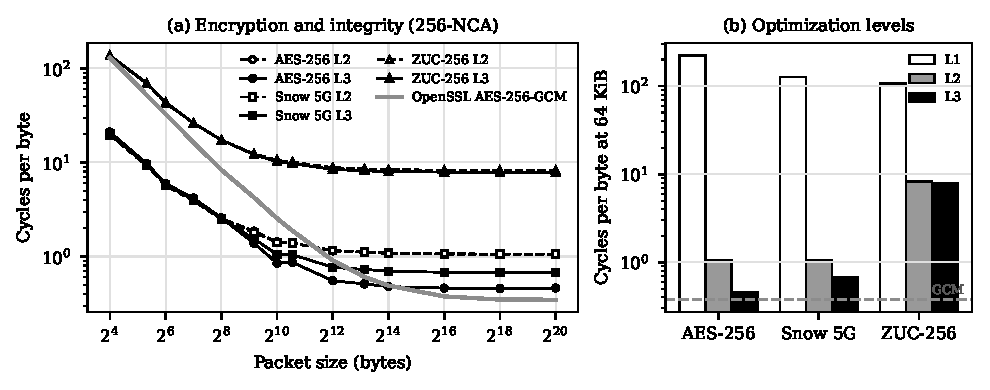
\includegraphics[width=\linewidth]{../figures/fig2_zen4.pdf}
\caption{Cloud tier (Zen~4, one core at 3.8~GHz). (a) Cycles per byte of 256-NCA against packet size at L2 and L3, with OpenSSL AES-256-GCM. (b) Cycles per byte at 64~KiB at L1, L2 and L3; the dashed line marks AES-256-GCM. Script: \texttt{paper/figures/fig2\_zen4.py}.}
\label{fig:s-zen4}
\vspace{10pt}
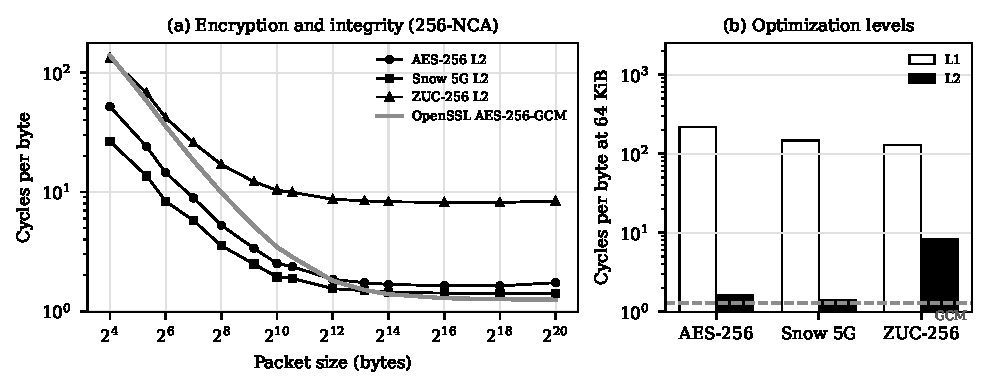
\includegraphics[width=\linewidth]{../figures/fig3_pi5.pdf}
\caption{Edge tier (Pi~5, one core at 2.4~GHz). (a) Cycles per byte of 256-NCA against packet size at L2, with OpenSSL AES-256-GCM. (b) Cycles per byte at 64~KiB at L1 and L2. Script: \texttt{paper/figures/fig3\_pi5.py}.}
\label{fig:s-pi5}
\vspace{10pt}
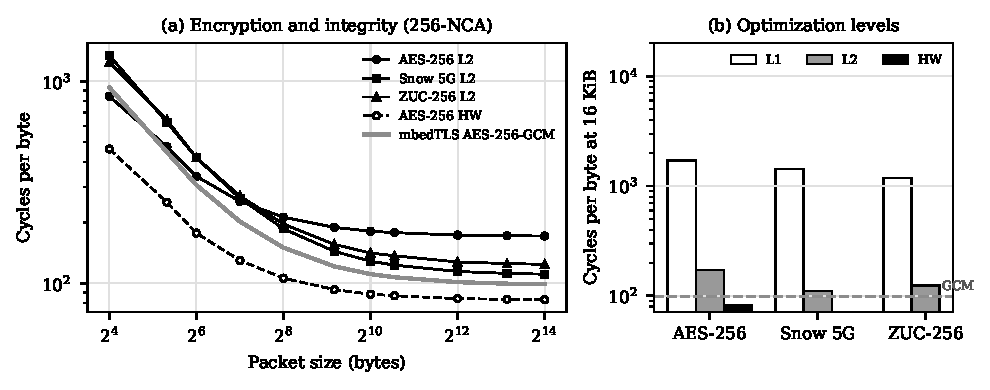
\includegraphics[width=\linewidth]{../figures/fig4_esp32.pdf}
\caption{Device tier (ESP32, one core at 240~MHz). (a) Cycles per byte of 256-NCA against packet size at L2 and HW, with mbedTLS AES-256-GCM. (b) Cycles per byte at 16~KiB at L1, L2 and HW. Script: \texttt{paper/figures/fig4\_esp32.py}.}
\label{fig:s-esp32}
\end{figure}

\subsection{Every packet size}

Table~\ref{tab:s-sizes} gives the cost of 256-NCA at every measured size on the three processors, for the fastest level of each set. These values feed Fig.~6 of the main paper.

\begin{table*}[p]
\centering
\caption{256-NCA cycles per packet at every measured size, with a 16-byte tag and no associated data. Zen~4 uses L2 below 512 bytes and L3 from 512 bytes; the Pi~5 uses L2; the ESP32 uses HW and L2. GCM is OpenSSL AES-256-GCM on the servers and mbedTLS AES-256-GCM on the ESP32. Sources: the three \texttt{*\_final*.csv} files of Table~\ref{tab:s-zen4} to Table~\ref{tab:s-esp32}.}
\label{tab:s-sizes}
\scriptsize
\setlength{\tabcolsep}{2.6pt}
\resizebox{\textwidth}{!}{%
\begin{tabular}{@{}r rrrr rrrr rrrrr@{}}
\toprule
Bytes & \multicolumn{4}{c}{Cloud: Zen 4} & \multicolumn{4}{c}{Edge: Pi 5} & \multicolumn{5}{c}{Device: ESP32} \\
\cmidrule(lr){2-5}\cmidrule(lr){6-9}\cmidrule(l){10-14}
 & AES-256 & Snow 5G & ZUC-256 & GCM & AES-256 & Snow 5G & ZUC-256 & GCM & AES HW & AES-256 & Snow 5G & ZUC-256 & GCM \\
\midrule
0 & 256 & 234 & 2{,}088 & 1{,}957 & 721 & 342 & 2{,}045 & 2{,}147 & 5{,}871 & 10{,}523 & 19{,}326 & 18{,}595 & 13{,}326 \\
16 & 322 & 314 & 2{,}202 & 2{,}071 & 831 & 424 & 2{,}121 & 2{,}231 & 7{,}395 & 13{,}482 & 21{,}501 & 19{,}930 & 14{,}920 \\
40 & 372 & 369 & 2{,}760 & 2{,}085 & 955 & 543 & 2{,}697 & 2{,}314 & 10{,}080 & 18{,}985 & 25{,}080 & 25{,}713 & 17{,}863 \\
64 & 367 & 365 & 2{,}746 & 2{,}101 & 928 & 535 & 2{,}682 & 2{,}280 & 11{,}350 & 21{,}663 & 26{,}767 & 26{,}792 & 19{,}627 \\
128 & 527 & 500 & 3{,}360 & 2{,}102 & 1{,}141 & 737 & 3{,}303 & 2{,}342 & 16{,}621 & 32{,}572 & 33{,}746 & 34{,}637 & 25{,}906 \\
256 & 648 & 638 & 4{,}434 & 2{,}138 & 1{,}347 & 907 & 4{,}342 & 2{,}533 & 27{,}166 & 54{,}388 & 47{,}702 & 50{,}318 & 38{,}468 \\
576 & 798 & 889 & 6{,}997 & 2{,}450 & 1{,}939 & 1{,}434 & 7{,}018 & 2{,}968 & 53{,}639 & 109{,}068 & 82{,}965 & 89{,}784 & 69{,}868 \\
1024 & 871 & 1{,}080 & 10{,}431 & 2{,}605 & 2{,}575 & 1{,}980 & 10{,}567 & 3{,}530 & 90{,}544 & 185{,}425 & 131{,}814 & 144{,}672 & 113{,}830 \\
1500 & 1{,}299 & 1{,}569 & 14{,}598 & 2{,}820 & 3{,}538 & 2{,}828 & 14{,}888 & 4{,}268 & 130{,}274 & 267{,}452 & 184{,}594 & 205{,}483 & 160{,}817 \\
4 KiB & 2{,}261 & 3{,}142 & 34{,}566 & 3{,}719 & 7{,}577 & 6{,}327 & 35{,}552 & 7{,}372 & 344{,}284 & 709{,}856 & 468{,}992 & 522{,}619 & 415{,}294 \\
9000 & 4{,}598 & 6{,}556 & 73{,}389 & 5{,}452 & 15{,}618 & 13{,}388 & 75{,}787 & 13{,}573 & 750{,}095 & 1{,}549{,}576 & 1{,}008{,}384 & 1{,}127{,}991 & 897{,}116 \\
16 KiB & 7{,}825 & 11{,}436 & 131{,}137 & 8{,}036 & 27{,}454 & 23{,}630 & 135{,}384 & 22{,}733 & 1{,}360{,}248 & 2{,}808{,}704 & 1{,}818{,}771 & 2{,}035{,}464 & 1{,}622{,}105 \\
64 KiB & 30{,}214 & 44{,}475 & 517{,}421 & 24{,}670 & 107{,}270 & 92{,}943 & 535{,}642 & 84{,}306 & -- & -- & -- & -- & -- \\
256 KiB & 119{,}570 & 176{,}527 & 2{,}062{,}507 & 91{,}134 & 427{,}303 & 370{,}862 & 2{,}137{,}551 & 330{,}247 & -- & -- & -- & -- & -- \\
1024 KiB & 484{,}308 & 708{,}756 & 8{,}247{,}662 & 363{,}682 & 1{,}819{,}379 & 1{,}482{,}844 & 8{,}807{,}481 & 1{,}309{,}345 & -- & -- & -- & -- & -- \\
\bottomrule
\end{tabular}}
\end{table*}


\subsection{Share of the setup cost}

Fig.~\ref{fig:s-setup}, which also appears as Fig.~4 of the main paper, shows the share of the fixed setup in the total cost of one packet at L2. On Zen~4, for a 40-byte packet, setup makes up 69\% of the cost of 256-NCA5, 63\% for 256-NCA4 and 76\% for 256-NCA6, and 94\% for OpenSSL AES-256-GCM. At 1500 bytes, the share falls to 11 to 14\% for the 3GPP sets, but it stays at 69\% for AES-256-GCM. On the Pi~5, setup makes up 75\%, 63\% and 76\% of the cost of a 40-byte packet, and 93\% for AES-256-GCM. At 1500 bytes, the shares fall to 20\%, 12\% and 14\%, and to 50\% for AES-256-GCM. On the ESP32, setup makes up 55\% of the cost of 256-NCA5, 77\% for 256-NCA4 and 72\% for 256-NCA6 at 40 bytes, and 4 to 10\% at 1500 bytes. mbedTLS AES-256-GCM has the same shape, with 75\% and 8\%.

\begin{figure}[t]
\centering
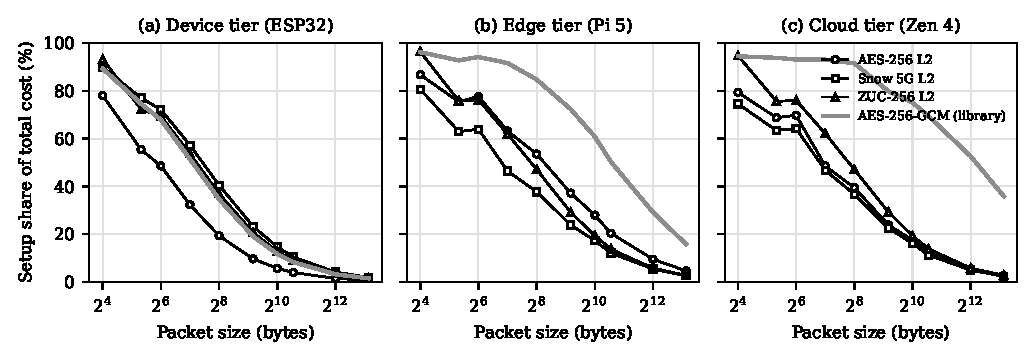
\includegraphics[width=\linewidth]{../figures/fig5_setup.pdf}
\caption{Share of the fixed setup cost in the total cost of 256-NCA at L2, against packet size. (a) ESP32. (b) Pi~5. (c) Zen~4. The grey line is AES-256-GCM in mbedTLS (a) or OpenSSL (b, c). Script: \texttt{paper/figures/fig3\_pi5.py}, which writes this figure as well.}
\label{fig:s-setup}
\end{figure}

\subsection{Multi-core scaling}

Tables~\ref{tab:s-mc-zen4} and~\ref{tab:s-mc-pi5} give the total throughput for every thread count, and Fig.~\ref{fig:s-mc} (Fig.~3 of the main paper) shows the speed-up at 1500 bytes. On eight Zen~4 cores at 64~KiB, AEGIS-256 reaches 697.1~Gbit/s and AES-256-GCM 605.7~Gbit/s. With all 16 logical cores, two threads share the vector and AES units of one core, and each thread needs 1.4 to 1.9 times more cycles per byte. On the Pi~5, two cores reach 93 to 100\% of twice the single-core throughput at 1500 and 65{,}536 bytes. On four cores, the core temperature stays below 72~$^\circ$C and the firmware reports no throttling. For 40-byte packets on four cores, the cycles per byte rise by 1 to 4\% for the 3GPP sets and by 21\% for OpenSSL AES-256-GCM. Table~\ref{tab:s-mc-fetch} compares the usual OpenSSL call with a cipher object fetched once per thread. With the usual call, ChaCha20-Poly1305 on eight cores reaches 3.7 times its single-core throughput at 1500 bytes. With the fetched object, it reaches 6.5 times at 1500 bytes and 4.4 times at 40 bytes.

\begin{table}[!htbp]
\centering
\caption{Multi-core throughput on Zen~4 in Gbit/s (16: both threads of all cores; Eff.: 8-core over 8$\times$ single-core). Source: \texttt{zen4\_mc.csv}.}
\label{tab:s-mc-zen4}
\footnotesize
\begin{tabular}{@{}>{\bfseries}l r r r r r r r@{}}
\toprule
\textbf{Algorithm} & \textbf{Bytes} & \multicolumn{5}{c}{\textbf{Threads}} & \textbf{Eff.} \\
\cmidrule(lr){3-7}
& & \textbf{1} & \textbf{2} & \textbf{4} & \textbf{8} & \textbf{16} & \textbf{(\%)} \\
\midrule
256-NCA5 (AES-256) & 40 & 3.11 & 6.14 & 10.5 & 22.4 & 31.4 & 90 \\
 & 1500 & 34.5 & 68.6 & 132.3 & 267.9 & 325.0 & 97 \\
 & 65536 & 64.9 & 127.7 & 251.1 & 505.7 & 544.7 & 97 \\
\addlinespace[2pt]
256-NCA4 (SNOW 5G) & 40 & 3.14 & 5.85 & 9.52 & 19.9 & 27.6 & 79 \\
 & 1500 & 28.5 & 56.5 & 108.8 & 220.0 & 257.9 & 96 \\
 & 65536 & 44.0 & 87.3 & 175.1 & 347.1 & 377.2 & 99 \\
\addlinespace[2pt]
256-NCA6 (ZUC-256) & 40 & 0.42 & 0.84 & 1.67 & 3.33 & 3.68 & 99 \\
 & 1500 & 3.07 & 6.12 & 12.2 & 24.2 & 27.1 & 98 \\
 & 65536 & 3.78 & 7.54 & 15.1 & 29.9 & 33.2 & 99 \\
\addlinespace[2pt]
OpenSSL AES-256-GCM & 40 & 0.58 & 0.87 & 1.17 & 0.92 & 1.09 & 20 \\
 & 1500 & 15.9 & 26.2 & 39.6 & 35.3 & 40.9 & 28 \\
 & 65536 & 79.3 & 154.0 & 307.6 & 605.7 & 657.9 & 96 \\
\addlinespace[2pt]
OpenSSL ChaCha20-Poly1305 & 40 & 0.41 & 0.64 & 1.00 & 0.96 & 1.08 & 29 \\
 & 1500 & 9.06 & 15.8 & 28.1 & 37.8 & 41.7 & 52 \\
 & 65536 & 29.6 & 58.8 & 117.1 & 233.1 & 280.6 & 98 \\
\addlinespace[2pt]
libaegis AEGIS-256 & 40 & 5.72 & 10.4 & 20.7 & 42.1 & 60.1 & 92 \\
 & 1500 & 63.7 & 121.9 & 241.9 & 487.1 & 694.7 & 96 \\
 & 65536 & 87.7 & 174.9 & 348.0 & 697.1 & 951.4 & 99 \\
\bottomrule
\end{tabular}
\end{table}

\begin{table}[!htbp]
\centering
\caption{Multi-core throughput on the Pi~5 in Gbit/s (Eff.: 4-core over 4$\times$ single-core). Source: \texttt{pi5\_mc.csv}.}
\label{tab:s-mc-pi5}
\footnotesize
\begin{tabular}{@{}>{\bfseries}l r r r r r@{}}
\toprule
\textbf{Algorithm} & \textbf{Bytes} & \multicolumn{3}{c}{\textbf{Threads}} & \textbf{Eff.} \\
\cmidrule(lr){3-5}
& & \textbf{1} & \textbf{2} & \textbf{4} & \textbf{(\%)} \\
\midrule
256-NCA5 (AES-256) & 40 & 0.82 & 1.58 & 2.88 & 88 \\
 & 1500 & 8.13 & 16.1 & 29.5 & 91 \\
 & 65536 & 11.7 & 23.3 & 43.8 & 93 \\
\addlinespace[2pt]
256-NCA4 (SNOW 5G) & 40 & 1.41 & 2.70 & 5.08 & 90 \\
 & 1500 & 10.2 & 20.1 & 36.7 & 90 \\
 & 65536 & 13.4 & 26.8 & 48.4 & 90 \\
\addlinespace[2pt]
256-NCA6 (ZUC-256) & 40 & 0.28 & 0.56 & 1.02 & 90 \\
 & 1500 & 1.93 & 3.84 & 7.06 & 92 \\
 & 65536 & 2.34 & 4.65 & 8.60 & 92 \\
\addlinespace[2pt]
OpenSSL AES-256-GCM & 40 & 0.31 & 0.54 & 0.94 & 76 \\
 & 1500 & 6.53 & 12.2 & 22.2 & 85 \\
 & 65536 & 14.8 & 29.5 & 54.5 & 92 \\
\addlinespace[2pt]
OpenSSL ChaCha20-Poly1305 & 40 & 0.23 & 0.42 & 0.73 & 80 \\
 & 1500 & 3.07 & 5.93 & 10.8 & 88 \\
 & 65536 & 5.55 & 11.0 & 20.1 & 91 \\
\addlinespace[2pt]
libaegis AEGIS-256 & 40 & 2.42 & 4.48 & 8.14 & 84 \\
 & 1500 & 19.2 & 37.5 & 69.0 & 90 \\
 & 65536 & 23.4 & 46.5 & 84.3 & 90 \\
\bottomrule
\end{tabular}
\end{table}

\begin{table}[p]
\centering
\caption{OpenSSL on Zen~4 with the usual call (\texttt{EVP\_aes\_256\_gcm()} per packet) and with a cipher object fetched once per thread (\texttt{EVP\_CIPHER\_fetch}); the key is set up for every packet in both cases: total Gbit/s over all threads, median of three 2-second runs. Threads go to separate physical cores first, and 16 uses both hardware threads of all eight cores. Eff.\ is the throughput on 8 cores divided by 8 times the single-core value. Source: \texttt{results/zen4/zen4\_mc\_ossl.csv}.}
\label{tab:s-mc-fetch}
\footnotesize
\begin{tabular}{@{}l r r r r r r r@{}}
\toprule
Algorithm & Bytes & \multicolumn{5}{c}{Threads} & Eff. \\
\cmidrule(lr){3-7}
 & & 1 & 2 & 4 & 8 & 16 & (\%) \\
\midrule
OpenSSL AES-256-GCM & 40 & 0.58 & 0.93 & 1.08 & 0.82 & 1.06 & 18 \\
 & 1500 & 15.8 & 27.6 & 37.9 & 31.5 & 39.6 & 25 \\
 & 65536 & 79.2 & 157.2 & 308.6 & 604.7 & 659.8 & 95 \\
\addlinespace[2pt]
AES-256-GCM, fetched & 40 & 0.91 & 1.66 & 2.56 & 3.09 & 3.66 & 42 \\
 & 1500 & 22.5 & 43.0 & 74.2 & 102.7 & 130.5 & 57 \\
 & 65536 & 82.6 & 164.9 & 325.9 & 642.2 & 685.5 & 97 \\
\addlinespace[2pt]
OpenSSL ChaCha20-Poly1305 & 40 & 0.41 & 0.66 & 0.96 & 0.85 & 1.04 & 26 \\
 & 1500 & 9.04 & 16.1 & 27.8 & 33.6 & 39.5 & 46 \\
 & 65536 & 29.6 & 59.0 & 117.5 & 233.3 & 280.8 & 99 \\
\addlinespace[2pt]
ChaCha20-Poly1305, fetched & 40 & 0.59 & 1.06 & 1.86 & 2.60 & 3.39 & 55 \\
 & 1500 & 11.1 & 21.2 & 39.6 & 71.4 & 96.5 & 81 \\
 & 65536 & 30.1 & 60.1 & 120.1 & 238.8 & 283.3 & 99 \\
\bottomrule
\end{tabular}
\end{table}


\begin{figure}[t]
\centering
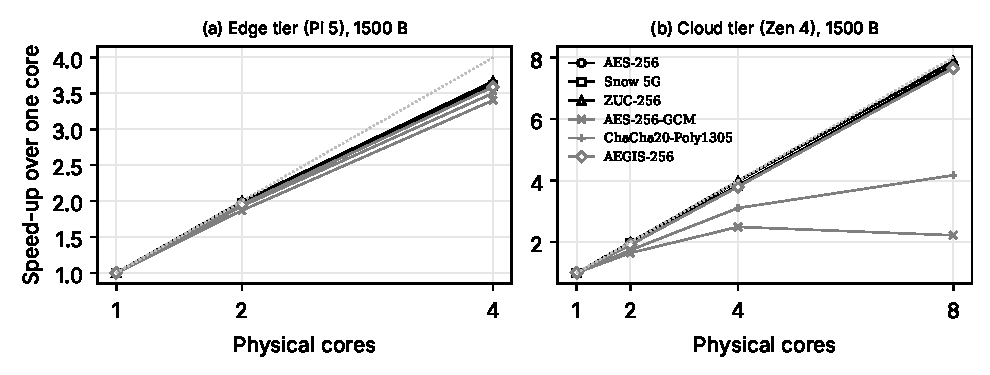
\includegraphics[width=\linewidth]{figS5_mc.pdf}
\caption{Speed-up over one core for 1500-byte packets on separate physical cores. The dotted line is ideal scaling. Data: \texttt{results/pi5/pi5\_mc.csv} and \texttt{results/zen4/zen4\_mc.csv}; script: \texttt{make\_tables.py}.}
\label{fig:s-mc}
\end{figure}

\subsection{Energy}

Table~\ref{tab:s-energy} extends Table~4 of the main paper. It adds the sum of all rails, the energy per packet, the idle and added power, the spread of the three repetitions and the highest core temperature. The 3GPP sets and AES-256-GCM come from the first energy run, and ChaCha20-Poly1305 and AEGIS-256 from a second run with the same method. The idle power of the core rail lies between 1.67 and 1.82~W in the first run and between 1.64 and 1.70~W in the second.

\begin{table}[!htbp]
\centering
\caption{Energy on one Pi~5 core at 2.4~GHz (median of three runs; spread: (max $-$ min)/median). Sources: \texttt{pi5\_energy.csv}, \texttt{pi5\_energy\_ref.csv}.}
\label{tab:s-energy}
\footnotesize
\begin{tabular}{@{}>{\bfseries}l r r r r r r r r@{}}
\toprule
\textbf{Algorithm} & \textbf{Bytes} & \textbf{nJ/B} & \textbf{nJ/B} & \textbf{$\mu$J/pkt} & \textbf{Idle} & \textbf{$\Delta P$} & \textbf{Spread} & \textbf{Max} \\
& & \textbf{core} & \textbf{all rails} & \textbf{core} & \textbf{(W)} & \textbf{(W)} & \textbf{(\%)} & \textbf{$^\circ$C} \\
\midrule
SNOW 5G (NCA4), L2 & 40 & 7.03 & 7.04 & 0.281 & 1.71 & 1.23 & 1.9 & 57.6 \\
 & 1500 & 0.98 & 0.93 & 1.469 & 1.73 & 1.24 & 1.3 & 56.0 \\
 & 65536 & 0.84 & 0.87 & 54.919 & 1.75 & 1.40 & 3.3 & 57.1 \\
\addlinespace[2pt]
AES-256 (NCA5), L2 & 40 & 8.30 & 9.05 & 0.332 & 1.78 & 0.83 & 7.0 & 56.0 \\
 & 1500 & 1.05 & 0.99 & 1.580 & 1.74 & 1.07 & 3.9 & 56.5 \\
 & 65536 & 0.86 & 0.85 & 56.341 & 1.76 & 1.25 & 7.6 & 57.1 \\
\addlinespace[2pt]
ZUC-256 (NCA6), L2 & 40 & 25.14 & 25.55 & 1.006 & 1.73 & 0.89 & 8.7 & 56.0 \\
 & 1500 & 3.70 & 3.56 & 5.544 & 1.72 & 0.89 & 15.1 & 57.6 \\
 & 65536 & 3.32 & 3.31 & 217.330 & 1.74 & 0.97 & 4.4 & 56.5 \\
\addlinespace[2pt]
AES-256-GCM, OpenSSL & 40 & 24.62 & 24.04 & 0.985 & 1.74 & 1.02 & 3.1 & 57.1 \\
 & 1500 & 1.31 & 1.26 & 1.971 & 1.76 & 1.11 & 6.2 & 57.6 \\
 & 65536 & 0.74 & 0.79 & 48.241 & 1.76 & 1.36 & 5.5 & 57.6 \\
\addlinespace[2pt]
ChaCha20-Poly1305, OpenSSL & 40 & 32.08 & 31.41 & 1.283 & 1.66 & 0.92 & 2.0 & 56.5 \\
 & 1500 & 2.83 & 2.78 & 4.242 & 1.69 & 1.07 & 3.5 & 58.7 \\
 & 65536 & 1.89 & 1.93 & 123.640 & 1.67 & 1.31 & 4.0 & 57.1 \\
\addlinespace[2pt]
AEGIS-256, libaegis & 40 & 4.43 & 4.27 & 0.177 & 1.67 & 1.31 & 1.1 & 58.7 \\
 & 1500 & 0.55 & 0.56 & 0.830 & 1.67 & 1.32 & 1.0 & 57.6 \\
 & 65536 & 0.48 & 0.52 & 31.615 & 1.68 & 1.46 & 3.5 & 58.2 \\
\bottomrule
\end{tabular}
\end{table}


\subsection{Hardware tier}

Table~\ref{tab:s-fpga} lists every out-of-context build, including the keystream generators built alone, and the board cycle counts of every timing packet. Built alone, the ZUC-256 generator is the smallest, with 355 slices at 120.2~MHz. The AES-256 generator with one round per clock uses 602 slices at 194.9~MHz, and with two rounds per clock 928 slices at 111.8~MHz. The Snow~5G generator with one AES round per clock uses 653 slices at 153.1~MHz, and with two rounds per clock 789 slices at 187.5~MHz. In the full AES-256 throughput engine, the doubled rounds double the dynamic power of the compact engine, but they raise the throughput by only 63\%. The engine therefore needs the most dynamic energy per byte.

\begin{table*}[!htbp]
\centering
\caption{All out-of-context builds on the XC7S25-1 ($f_{\max} = 1/(T - \mathrm{WNS})$; power: Vivado estimate, static 0.058~W). Source: \texttt{ooc\_final/reports/summary.csv}.}
\label{tab:s-fpga}
\footnotesize
\resizebox{\textwidth}{!}{%
\begin{tabular}{@{}>{\bfseries}l r r r r r r r r r r@{}}
\toprule
\textbf{Design} & \textbf{LUT} & \textbf{FF} & \textbf{Slice} & \textbf{BRAM} & \textbf{$T$ (ns)} & \textbf{WNS (ns)} & \textbf{$f_{\max}$ (MHz)} & \textbf{Dyn.\ W} & \textbf{Total W} & \textbf{Dyn.\ W} \\
& & & & & & & & \textbf{at $f_{\max}$} & \textbf{at $f_{\max}$} & \textbf{at 100 MHz} \\
\midrule
AES-256 generator, 1 round/clk & 1728 & 1162 & 602 & 0 & 5.20 & 0.068 & 194.9 & 0.107 & 0.165 & 0.056 \\
AES-256 generator, 2 rounds/clk & 2674 & 1161 & 928 & 0.5 & 8.80 & -0.142 & 111.8 & 0.215 & 0.273 & 0.189 \\
SNOW 5G generator, 1 AES round/clk & 2084 & 1674 & 653 & 0 & 6.10 & -0.433 & 153.1 & 0.089 & 0.147 & 0.054 \\
SNOW 5G generator, 2 AES rounds/clk & 2489 & 1801 & 789 & 0 & 5.15 & -0.184 & 187.5 & 0.138 & 0.196 & 0.071 \\
ZUC-256 generator & 972 & 826 & 355 & 0 & 8.05 & -0.268 & 120.2 & 0.047 & 0.105 & 0.038 \\
\midrule
256-NCA5 design A & 2981 & 2200 & 1015 & 0.5 & 6.05 & -0.247 & 158.8 & 0.118 & 0.176 & 0.072 \\
256-NCA5 design T & 5443 & 2205 & 1694 & 0.5 & 8.70 & -0.125 & 113.3 & 0.237 & 0.295 & 0.206 \\
256-NCA4 design A & 3293 & 2716 & 1101 & 0 & 6.50 & -0.135 & 150.7 & 0.096 & 0.154 & 0.062 \\
256-NCA4 design T & 4913 & 2717 & 1429 & 4 & 6.20 & -0.259 & 154.8 & 0.205 & 0.263 & 0.127 \\
256-NCA6 design A & 2394 & 1871 & 791 & 0 & 7.70 & -0.458 & 122.6 & 0.080 & 0.138 & 0.061 \\
256-NCA6 design T & 3810 & 1870 & 1085 & 0 & 7.80 & -0.108 & 126.5 & 0.110 & 0.168 & 0.085 \\
\bottomrule
\end{tabular}}

\vspace{6pt}
\resizebox{\textwidth}{!}{%
\begin{tabular}{@{}>{\bfseries}l r r r r r r r r r@{}}
\toprule
\textbf{Engine} & \multicolumn{5}{c}{\textbf{256-NCA cycles on the board}} & \textbf{NEA} & \textbf{NIA} & \multicolumn{2}{c}{\textbf{Latency at $f_{\max}$ (ns)}} \\
\cmidrule(lr){2-6}\cmidrule(l){9-10}
& \textbf{0 B} & \textbf{40 B} & \textbf{576 B} & \textbf{1500 B} & \textbf{16 KiB} & \textbf{16 KiB} & \textbf{1500 B} & \textbf{40 B} & \textbf{1500 B} \\
\midrule
256-NCA5 design A & 65 & 124 & 652 & 1580 & 16460 & 14340 & 1567 & 781 & 9950 \\
256-NCA5 design T & 32 & 54 & 285 & 691 & 7201 & 7172 & 406 & 477 & 6099 \\
256-NCA4 design A & 61 & 108 & 636 & 1564 & 16444 & 2084 & 1563 & 717 & 10378 \\
256-NCA4 design T & 30 & 41 & 173 & 405 & 4125 & 1044 & 404 & 265 & 2616 \\
256-NCA6 design A & 132 & 181 & 709 & 1637 & 16517 & 4197 & 1634 & 1476 & 13352 \\
256-NCA6 design T & 120 & 133 & 265 & 497 & 4217 & 4197 & 494 & 1051 & 3929 \\
\bottomrule
\end{tabular}}
\\[2pt]{\footnotesize Board cycle counts from \texttt{results/fpga/hw\_final/<design>/hwtest.txt} (127 of 127 packets match, 50~MHz).}
\end{table*}


\subsection{Timing-leakage tests}

Table~\ref{tab:s-ct} lists every dudect test with its number of measurements, the medians of the two classes and the source file. It includes the long Zen~4 L3 runs with 100 million measurements and the constant-time ZUC-256 runs on both processors. The constant-time ZUC-256 changes only the keystream generator, so 256-NIA6 uses it only for the setup. On the Pi~5, 256-NIA6 therefore costs 0.584 against 0.548 cycles per byte at 64~KiB, and 0.519 against 0.515 at 1~MiB, where the larger setup no longer matters (\texttt{results/pi5/pi5\_zucct.csv}). Its cost on Zen~4 is in \texttt{results/zen4/zen4\_zucct.csv}. The Zen~4 rerun of L1 Snow~5G with 20 million measurements, which gives $|t| = 17.6$ in Table~6 of the main paper, is in \texttt{results/zen4/zen4\_ct\_rerun.csv}. The same file holds a repeat of the two L3 data tests with 20 million measurements, which give 5.4 and 5.8.

{\scriptsize\setlength{\tabcolsep}{3.5pt}
\begin{longtable}{@{}>{\bfseries}l l l r l r r r r l l@{}}
\caption{All timing-leakage tests (Meas.: millions; medians in cycles; leak: $|t| > 10$; possible: $4.5 < |t| \le 10$). Source: \texttt{<platform>\_<file>.csv}.}
\label{tab:s-ct}\\
\toprule
\textbf{Platform} & \textbf{Level} & \textbf{Algorithm} & \textbf{Bytes} & \textbf{Test} & \textbf{Meas.} & \textbf{$|t|_{\max}$} & \textbf{Median 0} & \textbf{Median 1} & \textbf{Verdict} & \textbf{File} \\
\midrule
\endfirsthead
\toprule
\textbf{Platform} & \textbf{Level} & \textbf{Algorithm} & \textbf{Bytes} & \textbf{Test} & \textbf{Meas.} & \textbf{$|t|_{\max}$} & \textbf{Median 0} & \textbf{Median 1} & \textbf{Verdict} & \textbf{File} \\
\midrule
\endhead
Zen 4 & ctrl & early exit & 64 & key & 20 & 12628.52 & 114.1 & 874.3 & \textbf{leak} & \texttt{ct} \\
Zen 4 & ctrl & early exit & 64 & data & 20 & 0.58 & 874.3 & 874.2 & pass & \texttt{ct} \\
Zen 4 & ctrl & branch-free & 64 & key & 20 & 0.61 & 874.0 & 874.0 & pass & \texttt{ct} \\
Zen 4 & ctrl & branch-free & 64 & data & 20 & 0.16 & 874.0 & 874.0 & pass & \texttt{ct} \\
Zen 4 & L1 & 256-NCA5 & 64 & key & 3.03 & 34.54 & 23933.7 & 23937.9 & \textbf{leak} & \texttt{ct} \\
Zen 4 & L1 & 256-NCA5 & 64 & data & 3.04 & 1.68 & 23954.0 & 23954.2 & pass & \texttt{ct} \\
Zen 4 & L1 & 256-NCA4 & 64 & key & 3.46 & 4.51 & 20856.1 & 20856.7 & \emph{possible} & \texttt{ct} \\
Zen 4 & L1 & 256-NCA4 & 64 & data & 3.45 & 2.52 & 20885.0 & 20885.5 & pass & \texttt{ct} \\
Zen 4 & L1 & 256-NCA6 & 64 & key & 5.68 & 13.16 & 12377.1 & 12379.2 & \textbf{leak} & \texttt{ct} \\
Zen 4 & L1 & 256-NCA6 & 64 & data & 5.79 & 2.93 & 12268.4 & 12267.9 & pass & \texttt{ct} \\
Zen 4 & L2 & 256-NCA5 & 64 & key & 20 & 1.03 & 494.0 & 494.0 & pass & \texttt{ct} \\
Zen 4 & L2 & 256-NCA5 & 64 & data & 20 & 0.65 & 494.0 & 494.0 & pass & \texttt{ct} \\
Zen 4 & L2 & 256-NCA4 & 64 & key & 20 & 1.35 & 456.0 & 456.0 & pass & \texttt{ct} \\
Zen 4 & L2 & 256-NCA4 & 64 & data & 20 & 1.39 & 456.0 & 456.0 & pass & \texttt{ct} \\
Zen 4 & L2 & 256-NCA6 & 64 & key & 20 & 127.75 & 2860.9 & 2862.2 & \textbf{leak} & \texttt{ct} \\
Zen 4 & L2 & 256-NCA6 & 64 & data & 20 & 1.53 & 2864.2 & 2864.3 & pass & \texttt{ct} \\
Zen 4 & L3 & 256-NCA5 & 1024 & key & 20 & 1.91 & 988.0 & 988.0 & pass & \texttt{ct} \\
Zen 4 & L3 & 256-NCA5 & 1024 & data & 20 & 5.44 & 988.0 & 988.0 & \emph{possible} & \texttt{ct} \\
Zen 4 & L3 & 256-NCA4 & 1024 & key & 20 & 2.88 & 1216.0 & 1216.0 & pass & \texttt{ct} \\
Zen 4 & L3 & 256-NCA4 & 1024 & data & 20 & 7.83 & 1216.1 & 1216.1 & \emph{possible} & \texttt{ct} \\
Zen 4 & L3 & 256-NCA6 & 1024 & key & 6.17 & 101.49 & 10688.6 & 10689.1 & \textbf{leak} & \texttt{ct} \\
Zen 4 & L3 & 256-NCA6 & 1024 & data & 6.34 & 1.89 & 10698.2 & 10698.3 & pass & \texttt{ct} \\
Zen 4 & base & OpenSSL-AES-256-GCM & 64 & key & 20 & 2.20 & 2168.1 & 2168.0 & pass & \texttt{ct} \\
Zen 4 & base & OpenSSL-AES-256-GCM & 64 & data & 20 & 2.42 & 2165.8 & 2165.8 & pass & \texttt{ct} \\
Zen 4 & base & OpenSSL-ChaCha20-Poly1305 & 64 & key & 12.42 & 1.31 & 2962.7 & 2962.7 & pass & \texttt{ct} \\
Zen 4 & base & OpenSSL-ChaCha20-Poly1305 & 64 & data & 13.08 & 1.66 & 2953.0 & 2952.8 & pass & \texttt{ct} \\
Zen 4 & base & libaegis-AEGIS-256 & 64 & key & 20 & 0.26 & 268.0 & 268.0 & pass & \texttt{ct} \\
Zen 4 & base & libaegis-AEGIS-256 & 64 & data & 20 & 1.69 & 267.7 & 267.8 & pass & \texttt{ct} \\
\midrule
Zen 4 & L1 & 256-NCA4 & 64 & key & 20 & 17.59 & 21031.6 & 21032.8 & \textbf{leak} & \texttt{ct\_rerun} \\
Zen 4 & L1 & 256-NCA4 & 64 & data & 20 & 1.74 & 21058.9 & 21059.1 & pass & \texttt{ct\_rerun} \\
Zen 4 & L3 & 256-NCA5 & 1024 & key & 20 & 3.00 & 988.3 & 988.3 & pass & \texttt{ct\_rerun} \\
Zen 4 & L3 & 256-NCA5 & 1024 & data & 20 & 5.42 & 988.2 & 988.3 & \emph{possible} & \texttt{ct\_rerun} \\
Zen 4 & L3 & 256-NCA4 & 1024 & key & 20 & 1.39 & 1216.2 & 1216.2 & pass & \texttt{ct\_rerun} \\
Zen 4 & L3 & 256-NCA4 & 1024 & data & 20 & 5.83 & 1216.1 & 1216.1 & \emph{possible} & \texttt{ct\_rerun} \\
\midrule
Zen 4 & L3 & 256-NCA5 & 1024 & key & 100 & 2.51 & 988.2 & 988.3 & pass & \texttt{ct\_l3long} \\
Zen 4 & L3 & 256-NCA5 & 1024 & data & 100 & 9.69 & 988.7 & 988.7 & \emph{possible} & \texttt{ct\_l3long} \\
Zen 4 & L3 & 256-NCA4 & 1024 & key & 100 & 9.11 & 1216.5 & 1216.5 & \emph{possible} & \texttt{ct\_l3long} \\
Zen 4 & L3 & 256-NCA4 & 1024 & data & 100 & 13.05 & 1216.0 & 1216.0 & \textbf{leak} & \texttt{ct\_l3long} \\
\midrule
Zen 4 & L2 & 256-NCA6 & 64 & key & 20 & 190.89 & 2922.9 & 2919.5 & \textbf{leak} & \texttt{ct\_zuc} \\
Zen 4 & L2 & 256-NCA6 & 64 & data & 20 & 1.61 & 2932.5 & 2932.5 & pass & \texttt{ct\_zuc} \\
Zen 4 & L2ct & 256-NCA6 & 64 & key & 20 & 1.77 & 3068.7 & 3068.7 & pass & \texttt{ct\_zuc} \\
Zen 4 & L2ct & 256-NCA6 & 64 & data & 20 & 2.22 & 3105.8 & 3105.7 & pass & \texttt{ct\_zuc} \\
Zen 4 & L3 & 256-NCA6 & 1024 & key & 20 & 536.18 & 10672.1 & 10662.6 & \textbf{leak} & \texttt{ct\_zuc} \\
Zen 4 & L3 & 256-NCA6 & 1024 & data & 20 & 2.67 & 10639.2 & 10639.2 & pass & \texttt{ct\_zuc} \\
Zen 4 & L3ct & 256-NCA6 & 1024 & key & 20 & 1.96 & 11396.8 & 11396.6 & pass & \texttt{ct\_zuc} \\
Zen 4 & L3ct & 256-NCA6 & 1024 & data & 20 & 0.96 & 11398.5 & 11398.5 & pass & \texttt{ct\_zuc} \\
\midrule
Pi 5 & ctrl & early exit & 64 & key & 15.17 & 13121.90 & 109.7 & 842.2 & \textbf{leak} & \texttt{ct} \\
Pi 5 & ctrl & early exit & 64 & data & 13.9 & 0.95 & 834.5 & 834.5 & pass & \texttt{ct} \\
Pi 5 & ctrl & branch-free & 64 & key & 13.63 & 2.13 & 829.6 & 829.6 & pass & \texttt{ct} \\
Pi 5 & ctrl & branch-free & 64 & data & 13.92 & 2.44 & 829.6 & 829.6 & pass & \texttt{ct} \\
Pi 5 & L1 & 256-NCA5 & 64 & key & 1.84 & 21.03 & 23085.3 & 23087.8 & \textbf{leak} & \texttt{ct} \\
Pi 5 & L1 & 256-NCA5 & 64 & data & 1.84 & 1.63 & 23085.4 & 23085.1 & pass & \texttt{ct} \\
Pi 5 & L1 & 256-NCA4 & 64 & key & 1.89 & 16.23 & 22376.4 & 22378.6 & \textbf{leak} & \texttt{ct} \\
Pi 5 & L1 & 256-NCA4 & 64 & data & 1.9 & 2.28 & 22365.9 & 22365.8 & pass & \texttt{ct} \\
Pi 5 & L1 & 256-NCA6 & 64 & key & 2.78 & 55.31 & 14409.6 & 14414.3 & \textbf{leak} & \texttt{ct} \\
Pi 5 & L1 & 256-NCA6 & 64 & data & 2.78 & 0.84 & 14416.6 & 14416.5 & pass & \texttt{ct} \\
Pi 5 & L2 & 256-NCA5 & 64 & key & 11.78 & 1.30 & 1278.8 & 1278.8 & pass & \texttt{ct} \\
Pi 5 & L2 & 256-NCA5 & 64 & data & 11.88 & 1.69 & 1278.6 & 1278.6 & pass & \texttt{ct} \\
Pi 5 & L2 & 256-NCA4 & 64 & key & 13.09 & 1.17 & 895.2 & 895.2 & pass & \texttt{ct} \\
Pi 5 & L2 & 256-NCA4 & 64 & data & 13.2 & 2.16 & 894.9 & 894.9 & pass & \texttt{ct} \\
Pi 5 & L2 & 256-NCA6 & 64 & key & 8.19 & 13.21 & 3038.1 & 3038.1 & \textbf{leak} & \texttt{ct} \\
Pi 5 & L2 & 256-NCA6 & 64 & data & 8.25 & 3.06 & 3039.9 & 3040.0 & pass & \texttt{ct} \\
Pi 5 & base & OpenSSL-AES-256-GCM & 64 & key & 8.09 & 1.52 & 3026.3 & 3026.3 & pass & \texttt{ct} \\
Pi 5 & base & OpenSSL-AES-256-GCM & 64 & data & 8.23 & 1.56 & 3026.6 & 3026.5 & pass & \texttt{ct} \\
Pi 5 & base & OpenSSL-ChaCha20-Poly1305 & 64 & key & 7.12 & 1.34 & 3845.6 & 3845.6 & pass & \texttt{ct} \\
Pi 5 & base & OpenSSL-ChaCha20-Poly1305 & 64 & data & 7.21 & 1.53 & 3840.7 & 3840.8 & pass & \texttt{ct} \\
Pi 5 & base & libaegis-AEGIS-256 & 64 & key & 14.01 & 1.76 & 643.1 & 643.1 & pass & \texttt{ct} \\
Pi 5 & base & libaegis-AEGIS-256 & 64 & data & 14.19 & 2.01 & 643.2 & 643.1 & pass & \texttt{ct} \\
\midrule
Pi 5 & L2 & 256-NCA6 & 64 & key & 20 & 26.37 & 3036.6 & 3036.3 & \textbf{leak} & \texttt{ct\_zuc\_run1} \\
Pi 5 & L2 & 256-NCA6 & 64 & data & 20 & 1.82 & 3034.3 & 3034.3 & pass & \texttt{ct\_zuc\_run1} \\
\midrule
Pi 5 & L2 & 256-NCA6 & 64 & key & 20 & 110.80 & 3038.0 & 3036.7 & \textbf{leak} & \texttt{ct\_zuc} \\
Pi 5 & L2 & 256-NCA6 & 64 & data & 20 & 2.00 & 3034.8 & 3034.8 & pass & \texttt{ct\_zuc} \\
Pi 5 & L2ct & 256-NCA6 & 64 & key & 20 & 1.99 & 5853.9 & 5853.9 & pass & \texttt{ct\_zuc} \\
Pi 5 & L2ct & 256-NCA6 & 64 & data & 20 & 1.39 & 5854.2 & 5854.2 & pass & \texttt{ct\_zuc} \\
\bottomrule
\end{longtable}}


\subsection{Buffer placement}
\label{sec:s-layout}

Table~\ref{tab:s-layout} shows how much the position of the output buffer within a 4~KiB page changes the results. The effect is small at L2 on both processors, at most 0.5\%. At L3 on Zen~4, it reaches 6.4\%, with the largest change for AES-256 between 1500 and 4096 bytes. In an early run, before we fixed the layout, a larger buffer came from a different part of memory and changed the L3 AES-256 results by up to 17\%. All runs in the paper therefore use the same fixed layout.

\begin{table}[p]
\centering
\caption{Buffer-placement test: the output buffer is placed at five offsets within a 4~KiB page (0, 64, 1024, 2048 and 3072 bytes). The table gives the largest relative change of the median cycles over the five offsets, and the packet size where it occurs. Sources: \texttt{results/zen4/zen4\_layout.csv} and \texttt{results/pi5/pi5\_layout.csv}.}
\label{tab:s-layout}
\footnotesize
\begin{tabular}{@{}l l l r r@{}}
\toprule
Platform & Level & Algorithm & Max change (\%) & At bytes \\
\midrule
Zen 4 & L2 & 256-NCA4 & 0.2 & 1500 \\
Zen 4 & L2 & 256-NCA5 & 0.2 & 1500 \\
Zen 4 & L2 & 256-NEA5 & 0.4 & 65536 \\
Zen 4 & L3 & 256-NCA4 & 2.5 & 1500 \\
Zen 4 & L3 & 256-NCA5 & 6.0 & 4096 \\
Zen 4 & L3 & 256-NEA5 & 6.4 & 1500 \\
Pi 5 & L2 & 256-NCA4 & 0.5 & 4096 \\
Pi 5 & L2 & 256-NCA5 & 0.4 & 65536 \\
Pi 5 & L2 & 256-NEA5 & 0.2 & 4096 \\
\bottomrule
\end{tabular}
\end{table}


\section{Software and hardware environment}
\label{sec:s-env}

Table~\ref{tab:s-env} lists the environment of each platform. The files \texttt{*\_sysinfo*.txt} and \texttt{*\_info.txt} in \texttt{results/} record the full CPU description, the clock settings and the temperatures of each run.

\begin{table}[H]
\centering
\caption{Software and hardware environment. Sources: \texttt{results/zen4/zen4\_sysinfo\_ref.txt}, \texttt{results/pi5/pi5\_sysinfo\_ref.txt}, the header of \texttt{results/esp32/esp32\_run4\_log.txt}, and the Vivado reports.}
\label{tab:s-env}
\footnotesize
\begin{tabular}{@{}p{1.3cm} p{4.6cm} p{4.6cm} p{4.4cm}@{}}
\toprule
Platform & Processor & Software & Settings \\
\midrule
Zen 4 & AMD Ryzen 7 7700, 8 cores, 16 threads; 1~MiB L2 per core, 32~MiB L3; AVX-512, VAES, VPCLMULQDQ, VBMI & Ubuntu 24.04.5, Linux 7.0.0-38; GCC 13.3.0 \texttt{-O2}; OpenSSL 3.0.13; libaegis 0.9.1 (\texttt{-O3}) & Performance governor, 3.8~GHz fixed, boost off; process pinned to one core \\
Pi 5 & Broadcom BCM2712, 4 Cortex-A76 cores; 512~KiB L2 per core, 2~MiB L3; AES, PMULL, NEON & Debian 13; GCC 14.2.0 \texttt{-O2}; OpenSSL 3.5.7; libaegis 0.9.1 (\texttt{-O3}) & Performance governor, 2.4~GHz fixed; official Active Cooler (fan and heatsink) in the official case; temperature and throttling logged \\
ESP32 & ESP32-D0WD-V3, revision 3.1, two Xtensa LX6 cores at 240~MHz; 520~KiB SRAM; 4~MiB flash; AES engine & ESP-IDF 5.4.4; GCC 14.2.0 \texttt{-O2}; mbedTLS of ESP-IDF; libaegis 0.9.1 portable C & Radios off; benchmark task alone on core~1; measured code in IRAM \\
FPGA & Spartan-7 XC7S25-1 CSGA324 on Arty S7-25 (rev.~E) & Vivado 2025.2; VHDL-2008 & Out of context, default strategies; board test at 50~MHz from the 12~MHz clock \\
\bottomrule
\end{tabular}
\end{table}

\section{Code and data package}
\label{sec:s-artifact}

The package contains all source code, all raw measurement files, the scripts that turn them into the figures and tables, and the instructions to repeat every run. It is available at \repourl{} and archived with a permanent identifier at \zenodo{}. Its \texttt{README.md} gives a short start, and \texttt{docs/REPRODUCE.md} gives the full steps for each platform.

\subsection{Contents}

\begin{table}[H]
\centering
\caption{Layout of the code and data package.}
\label{tab:s-layout-repo}
\footnotesize
\begin{tabular}{@{}p{4.4cm} p{11.4cm}@{}}
\toprule
Folder & Contents \\
\midrule
\texttt{code/common} & AES-256 and POLYVAL reference code, and the shared 256-AEAD1 layer (L1) \\
\texttt{code/aes256set}, \texttt{snow5gset}, \texttt{zuc256set} & The three sets at L1, written from TS~35.243, 35.240 and 35.246; checks against the official test data \\
\texttt{code/l2x86}, \texttt{l3x86} & L2 (AES-NI, PCLMULQDQ, SSSE3) and L3 (AVX-512, VAES, VPCLMULQDQ) code; constant-time ZUC-256 (\texttt{zuc\_sbox\_ct.h}) \\
\texttt{code/l2arm} & L2 code for ARMv8 (AES, PMULL, NEON), including the constant-time ZUC-256 \\
\texttt{code/l2port} & Portable 32-bit L2 code, used on the ESP32 \\
\texttt{code/bench} & Benchmark (\texttt{bench}), multi-core (\texttt{mc}), timing-leakage (\texttt{ct}) and energy (\texttt{energy\_pi.py}) programs, with clock scripts \\
\texttt{code/esp32} & ESP-IDF project for the device tier, with the HW level and the reference schemes \\
\texttt{code/fpga} & VHDL engines, testbenches, test vectors, board wrapper and Vivado scripts \\
\texttt{code/third\_party/libaegis} & libaegis 0.9.1, unchanged, with its MIT licence \\
\texttt{results/} & Every raw CSV and log file of the paper and this supplement \\
\texttt{analysis/} & \texttt{build\_final\_csv.py}, which rebuilds and checks the merged result files \\
\texttt{paper/figures}, \texttt{paper/supplementary} & Scripts for every figure and every supplementary table \\
\texttt{docs/} & Reproduction guide, notes on the 3GPP reference code, and the run notes of each platform \\
\bottomrule
\end{tabular}
\end{table}

\subsection{Which script produces which result}

\begin{table}[H]
\centering
\caption{Source of every figure and table in the main paper and this supplement.}
\label{tab:s-map}
\footnotesize
\begin{tabular}{@{}p{2.6cm} p{5.6cm} p{7.4cm}@{}}
\toprule
Item & Script & Data \\
\midrule
Fig.~1 & \texttt{paper/figures/fig1\_aead1.py} & Drawing only \\
Fig.~2 & \texttt{paper/figures/fig2\_cpb.py} & \texttt{*\_final*.csv} of the three processors \\
Fig.~3 & \texttt{paper/supplementary/make\_tables.py} (as Fig.~S5) & \texttt{zen4\_mc.csv}, \texttt{pi5\_mc.csv} \\
Fig.~4 & \texttt{paper/figures/fig3\_pi5.py} (as Fig.~S4) & \texttt{*\_final*.csv} \\
Fig.~5 & \texttt{paper/figures/fig6\_fpga.py} & \texttt{fpga\_final.csv}, \texttt{ooc\_final/reports/*/} \texttt{utilization\_hier.rpt} \\
Fig.~6 & \texttt{paper/figures/fig8\_summary.py} & \texttt{*\_final*.csv}, \texttt{fpga\_final.csv}, \texttt{hw\_final/*/hwtest.txt} \\
Table~3 & Tables~\ref{tab:s-zen4}--\ref{tab:s-esp32} (\texttt{make\_tables.py}) & \texttt{*\_final*.csv}, \texttt{*\_base\_ref.csv}, \texttt{esp32\_run4.csv}, \texttt{esp32\_run5.csv} \\
Table~4 & Table~\ref{tab:s-energy} & \texttt{pi5\_energy.csv}, \texttt{pi5\_energy\_ref.csv} \\
Table~5 & \texttt{analysis/build\_final\_csv.py} & \texttt{fpga\_final.csv} \\
Table~6 & Table~\ref{tab:s-ct} & \texttt{*\_ct*.csv} \\
Multi-core text & Tables~\ref{tab:s-mc-zen4}--\ref{tab:s-mc-fetch} & \texttt{zen4\_mc.csv}, \texttt{zen4\_mc\_ossl.csv}, \texttt{pi5\_mc.csv} \\
Constant-time cost & -- & \texttt{zen4\_zucct.csv}, \texttt{pi5\_zucct.csv} \\
Figs.~S1--S4 & \texttt{fig2\_zen4.py}, \texttt{fig3\_pi5.py}, \texttt{fig4\_esp32.py} & \texttt{*\_final*.csv} \\
Fig.~S5, Tables~S1--S11 & \texttt{paper/supplementary/make\_tables.py} & As named in each caption \\
\bottomrule
\end{tabular}
\end{table}

\subsection{3GPP reference code}

The specifications TS~35.240, 35.243 and 35.246 include informative reference code in their annexes. We use it only to cross-check our L1 code on random inputs. The package does not contain this code, because 3GPP owns its copyright. Instead, the build extracts the annex code from the user's own copy of each specification with \texttt{code/common/extract\_annexb.py} and compiles it next to our code (\texttt{make verify}). The official test data are also not included. The scripts \texttt{test\_official.py} read them from the test-data documents. All these documents are free to download from the 3GPP website, and \texttt{docs/3GPP\_REFERENCE\_CODE.md} lists their exact versions. All other checks, including L2 and L3 against L1 and the ESP32 self-tests, run without these files.

\subsection{Licences}

Our code is released under the MIT licence, and our data and documentation under CC~BY~4.0. libaegis keeps its own MIT licence. ESP-IDF, mbedTLS and OpenSSL are not included; the build uses the versions installed on each platform.

\end{document}
